\documentclass[final]{beamer}

\usepackage{amsmath}
\usepackage{amssymb}
\usepackage{amsthm}
\usepackage{booktabs}
% \usepackage[figurename=(c),labelsep=space]{caption} % Hack
\usepackage{enumitem}
\usepackage{float}
\usepackage{geometry}
\usepackage{mathtools}
\usepackage{microtype}
\usepackage{nicefrac}
\usepackage{physics}
\usepackage{siunitx}
\usepackage{tikz}
\usepackage{xcolor}
\usepackage{pgffor}
\usepackage[orientation=landscape,size=custom,height=60.96,width=91.44,scale=1.0]{beamerposter}
\usepackage{adjustbox}
\usepackage{subcaption}

\graphicspath{{figs/}}

\usepackage[sfdefault,semibold]{libertine} % a bit lighter than Times--no osf in math
% \usepackage[libertine,vvarbb]{newtxmath}
\usepackage{eulervm}
\usepackage[scr=esstix,cal=boondoxo]{mathalfa}

\usetikzlibrary{arrows, shapes.misc, positioning, fit}
\tikzset{%
  invisible/.style={opacity=0,text opacity=0},
  visible on/.style={alt=#1{}{invisible}},
  alt/.code args={<#1>#2#3}{%
    \alt<#1>{\pgfkeysalso{#2}}{\pgfkeysalso{#3}} % \pgfkeysalso doesn't change the path
  },
}

\usecolortheme[snowy]{owl}
\usefonttheme{professionalfonts}
% \usefonttheme{serif}
\setbeamersize{text margin left=0pt, text margin right=0pt}
\setbeamertemplate{blocks}[rounded][shadow=true]
\setbeamercolor{title}{fg=white,bg=blue} % Temporary; tweak me!
% \setbeamercolor{block title}{bg=blue!70, fg=white}
\setbeamercolor{block title}{bg=blue, fg=white}
\setbeamercolor{block body}{bg=black!9}
\setbeamerfont{block title}{series=\bfseries}

% Hack a margin into blocks.
\newenvironment{mblock}[1]{%
  \begin{block}{#1}%
    \begin{adjustbox}{minipage=\linewidth-3ex, margin=1.5ex, center}}%
{\end{adjustbox}\end{block}}

% It's a hack, but it works.
\title{%
  \parbox{0.02\textwidth}{\hspace{-2.25ex}
\includegraphics[width=4.5ex]{nsf}\hfil}%
  \parbox{0.18\textwidth}{\small
    \textbf{Physics \textsc{Reu}: Summer 2020} \\
    Rensselaer Polytechnic Institute
  }
  \parbox{0.55\textwidth}{\Huge
    Understanding visual complexity with statistical physics
  }
  \parbox{0.20\textwidth}{\hfill
    Alex Striff \& Vincent Meunier
  }
}
\author{}
\date{}

\begin{document}
\begin{frame}[t]{}
  \vspace{-8pt}
  \begin{beamercolorbox}{}
    \maketitle
  \end{beamercolorbox}
  \vspace{-1.5in}
  \centering
  \begin{tikzpicture}[visible on=<+->]
  \node at (0,0) {%
  \begin{tikzpicture}[
    visible on=<+->,
    x=7cm,
    y=7cm,
    cclip/.style = {transparent, circle, minimum size=5cm, outer sep=6pt},
    clabel/.style = {text opacity=1, inner sep=0pt, text=white, font=\bfseries, align=center}
    ]
    \node[visible on=<.(14)->, circle, fill=black!10, inner sep=0pt,
      outer sep=0pt, minimum size=19cm]
      (visual world) at (0,0) {};
    \node[visible on=<.(14)->, below=of visual world, inner sep=0pt, outer sep=0pt, text
      width=21cm, align=center] {%
        \textcolor{green}{We} cannot \textcolor{red}{directly percieve} the
        true nature of the world, but we can form models to
        \textcolor{orange}{indirectly percieve} nature. A model must represent
        nature, while still being something we can readily look at and use to
        guide thought. \textbf{What are good models of how nature looks to
        us?}
      };
    \begin{scope}[visible on=<.->]
      \node[cclip] (natural) at (120:1) {};
      \clip (natural) circle (2.5cm)
      node {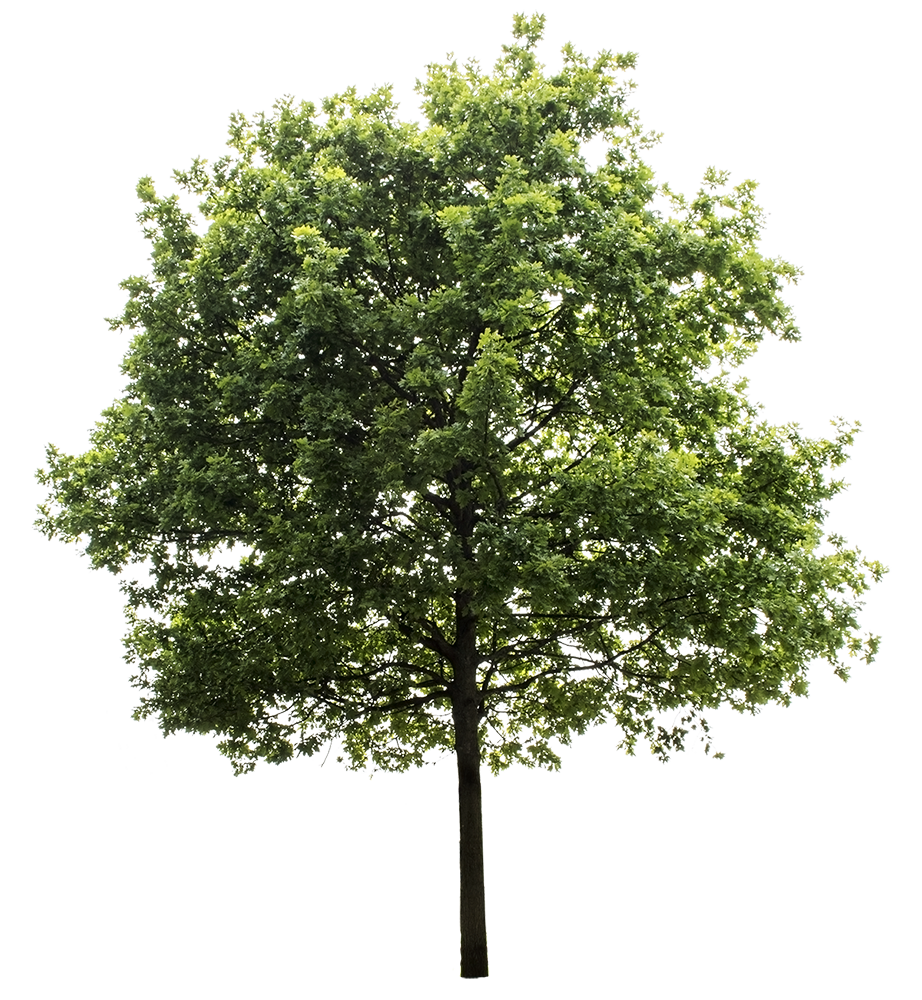
\includegraphics[width=5cm]{tree-natural}};
      \node[clabel] at (natural) {Natural};
    \end{scope}
    \begin{scope}[visible on=<.(1)->]
      \node[cclip] (seen) at (0,0) {};
      \clip (seen) circle (2.5cm)
      node {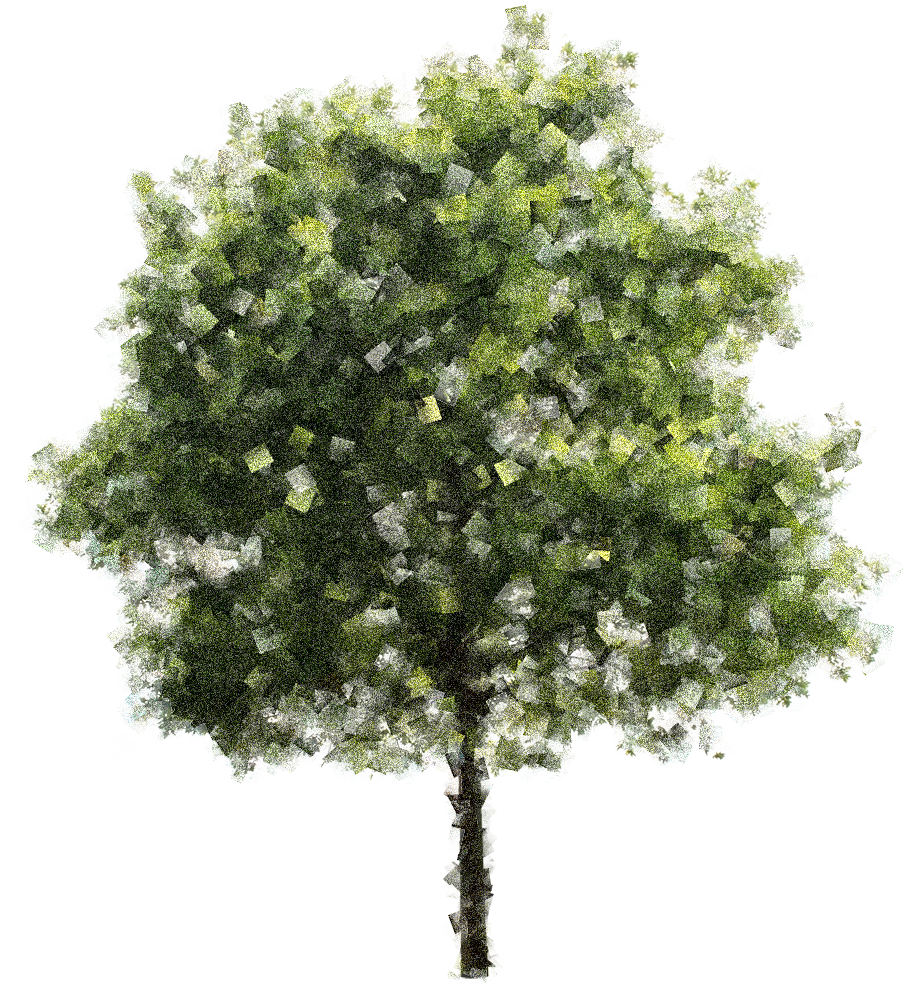
\includegraphics[width=5cm]{tree-seen}};
      \node[clabel] at (seen) {Sight};
    \end{scope}
    \begin{scope}[visible on=<.(2)->]
      \node[cclip] (cartoon) at (0:1) {};
      \clip (cartoon) circle (2.5cm)
      node {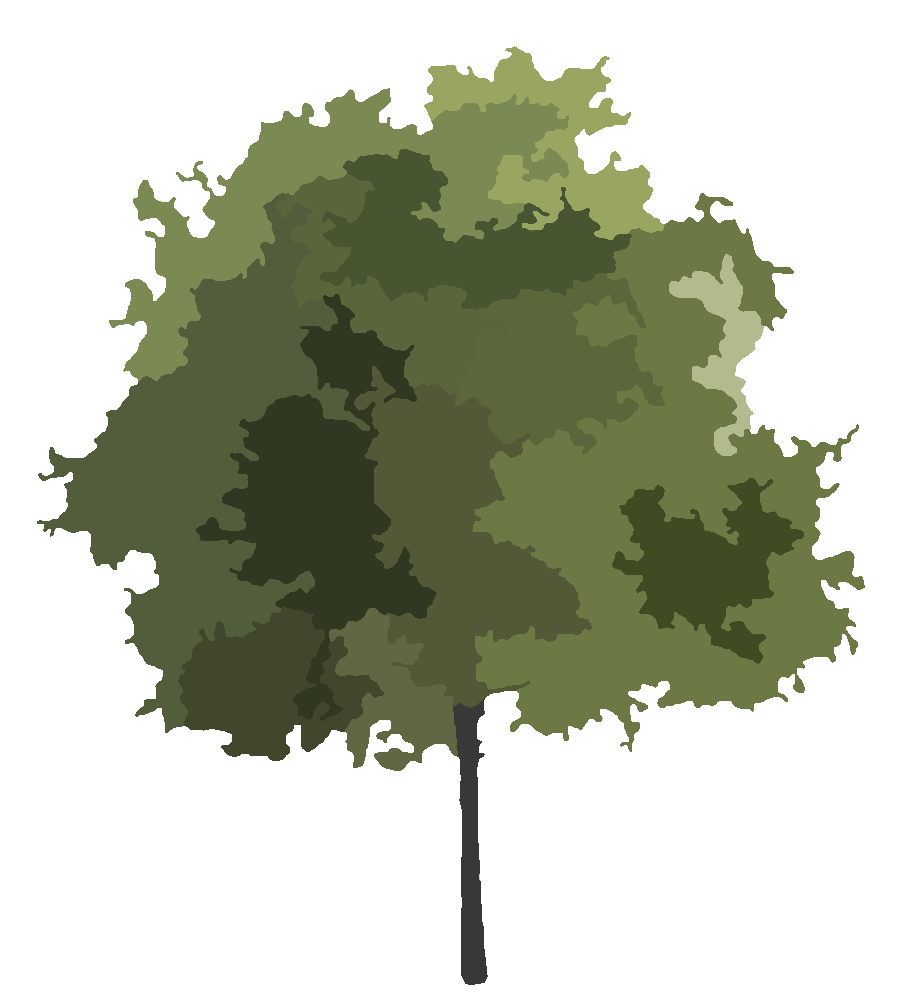
\includegraphics[width=5cm]{tree-cartoon}};
      \node[clabel] at (cartoon) {Thought};
    \end{scope}
    \begin{scope}[visible on=<.(7)->]
      \node[cclip] (bitmap) at (-120:1) {};
      \clip (bitmap) circle (2.5cm)
      node {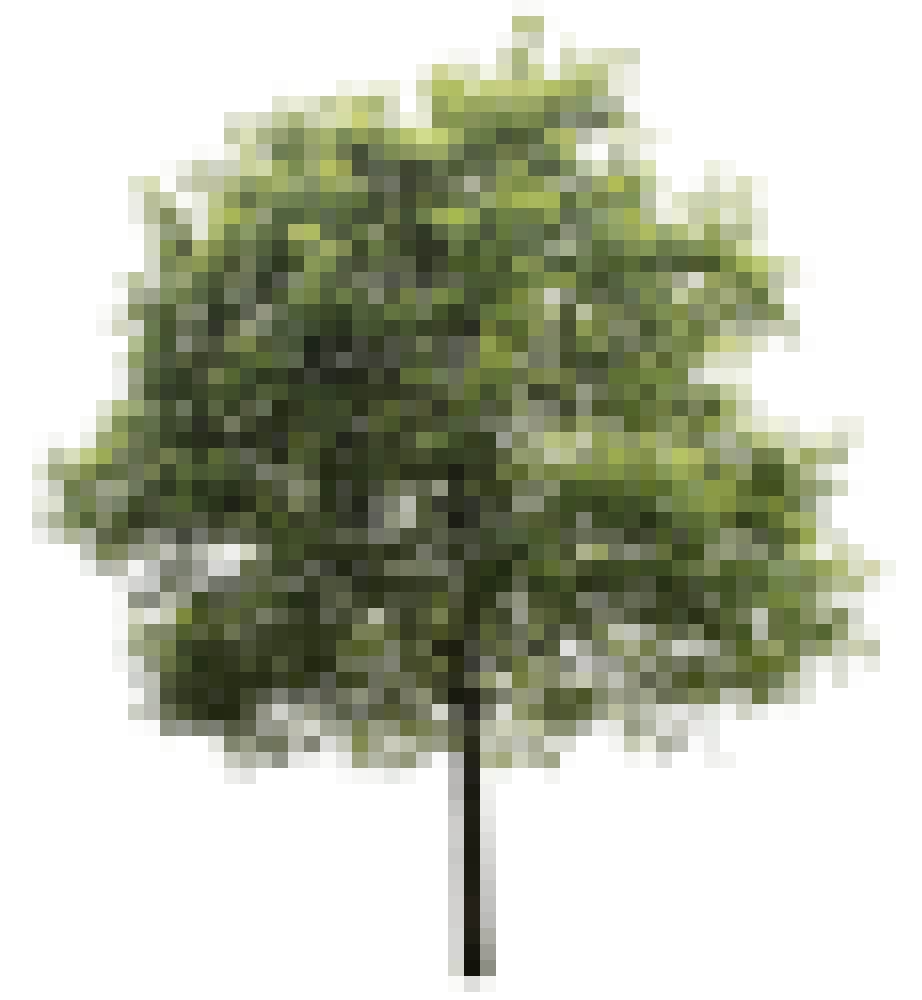
\includegraphics[width=5cm]{tree-bitmap}};
      \node[clabel] at (bitmap) {Model};
    \end{scope}
    \begin{scope}[->, line width=3pt]
      \begin{scope}[green]
        \draw[visible on=<.(1)->] (natural) to[bend right=15] node[below,sloped]{Look} (seen);
        \draw[visible on=<.(2)->] (seen) to[bend left=15] node[above]{Percieve} (cartoon);
        \draw[visible on=<.(3)->] (cartoon) to[bend left=15] node[below]{Reflect} (seen);
        \draw[visible on=<.(9)->] (bitmap) to[bend left=15] node[above,sloped]{Look} (seen);
      \end{scope}
      \begin{scope}[orange]
        \draw[visible on=<.(8)->] (natural) to[bend right=45] node[above,sloped,rotate=180]{Represent} (bitmap);
        \draw[visible on=<.(10)->] (seen) to[bend left=15] node[below,sloped]{Rep.} (bitmap);
        \draw[visible on=<.(11)->] (bitmap) to[bend right=45] node[above,sloped]{Learn} (cartoon);
        \draw[visible on=<.(12)->] (cartoon)  to[bend left=25] node[above,sloped]{Abstract} (bitmap);
        \draw[visible on=<.(13)->] (bitmap) to[bend left=25] node[above,sloped]{Generate} (natural);
      \end{scope}
      \begin{scope}[red]
        \draw[visible on=<.(4)->] (natural) to[bend left=25] node[above,sloped]{Omniscience} (cartoon);
        \draw[visible on=<.(5)->] (cartoon) to[bend right=45] node[above,sloped]{Physics} (natural);
        \draw[visible on=<.(6)->] (seen) to[bend right=15] node[above,sloped]{Psych.} (natural);
      \end{scope}
    \end{scope}
    \addtocounter{beamerpauses}{14}
  \end{tikzpicture}
  };

  \node[xshift=0.333333\textwidth,yshift=0.25\textheight] at (visual world) {%
  \begin{tikzpicture}[
    visible on=<+->,
    x=7cm,
    y=7cm,
    cclip/.style = {transparent, circle, minimum size=5cm, outer sep=6pt},
    clabel/.style = {text opacity=1, inner sep=0pt, text=white, font=\bfseries}
    ]
    \node[circle, fill=black!10, inner sep=0pt,
      outer sep=0pt, minimum size=15cm]
      (visual complexity) at (0,0) {};
    \node[below=of visual complexity, inner sep=0pt, outer sep=0pt, text
      width=16cm, align=center] {%
        \textbf{Visual complexity} arises in many ways. Computational models of
        these phenomena are the bricks that build up the structure of an image.
      };
    \begin{scope}
      \node[cclip] (ifs) at (-135:0.625) {};
      \clip (ifs) circle (2.5cm)
      node {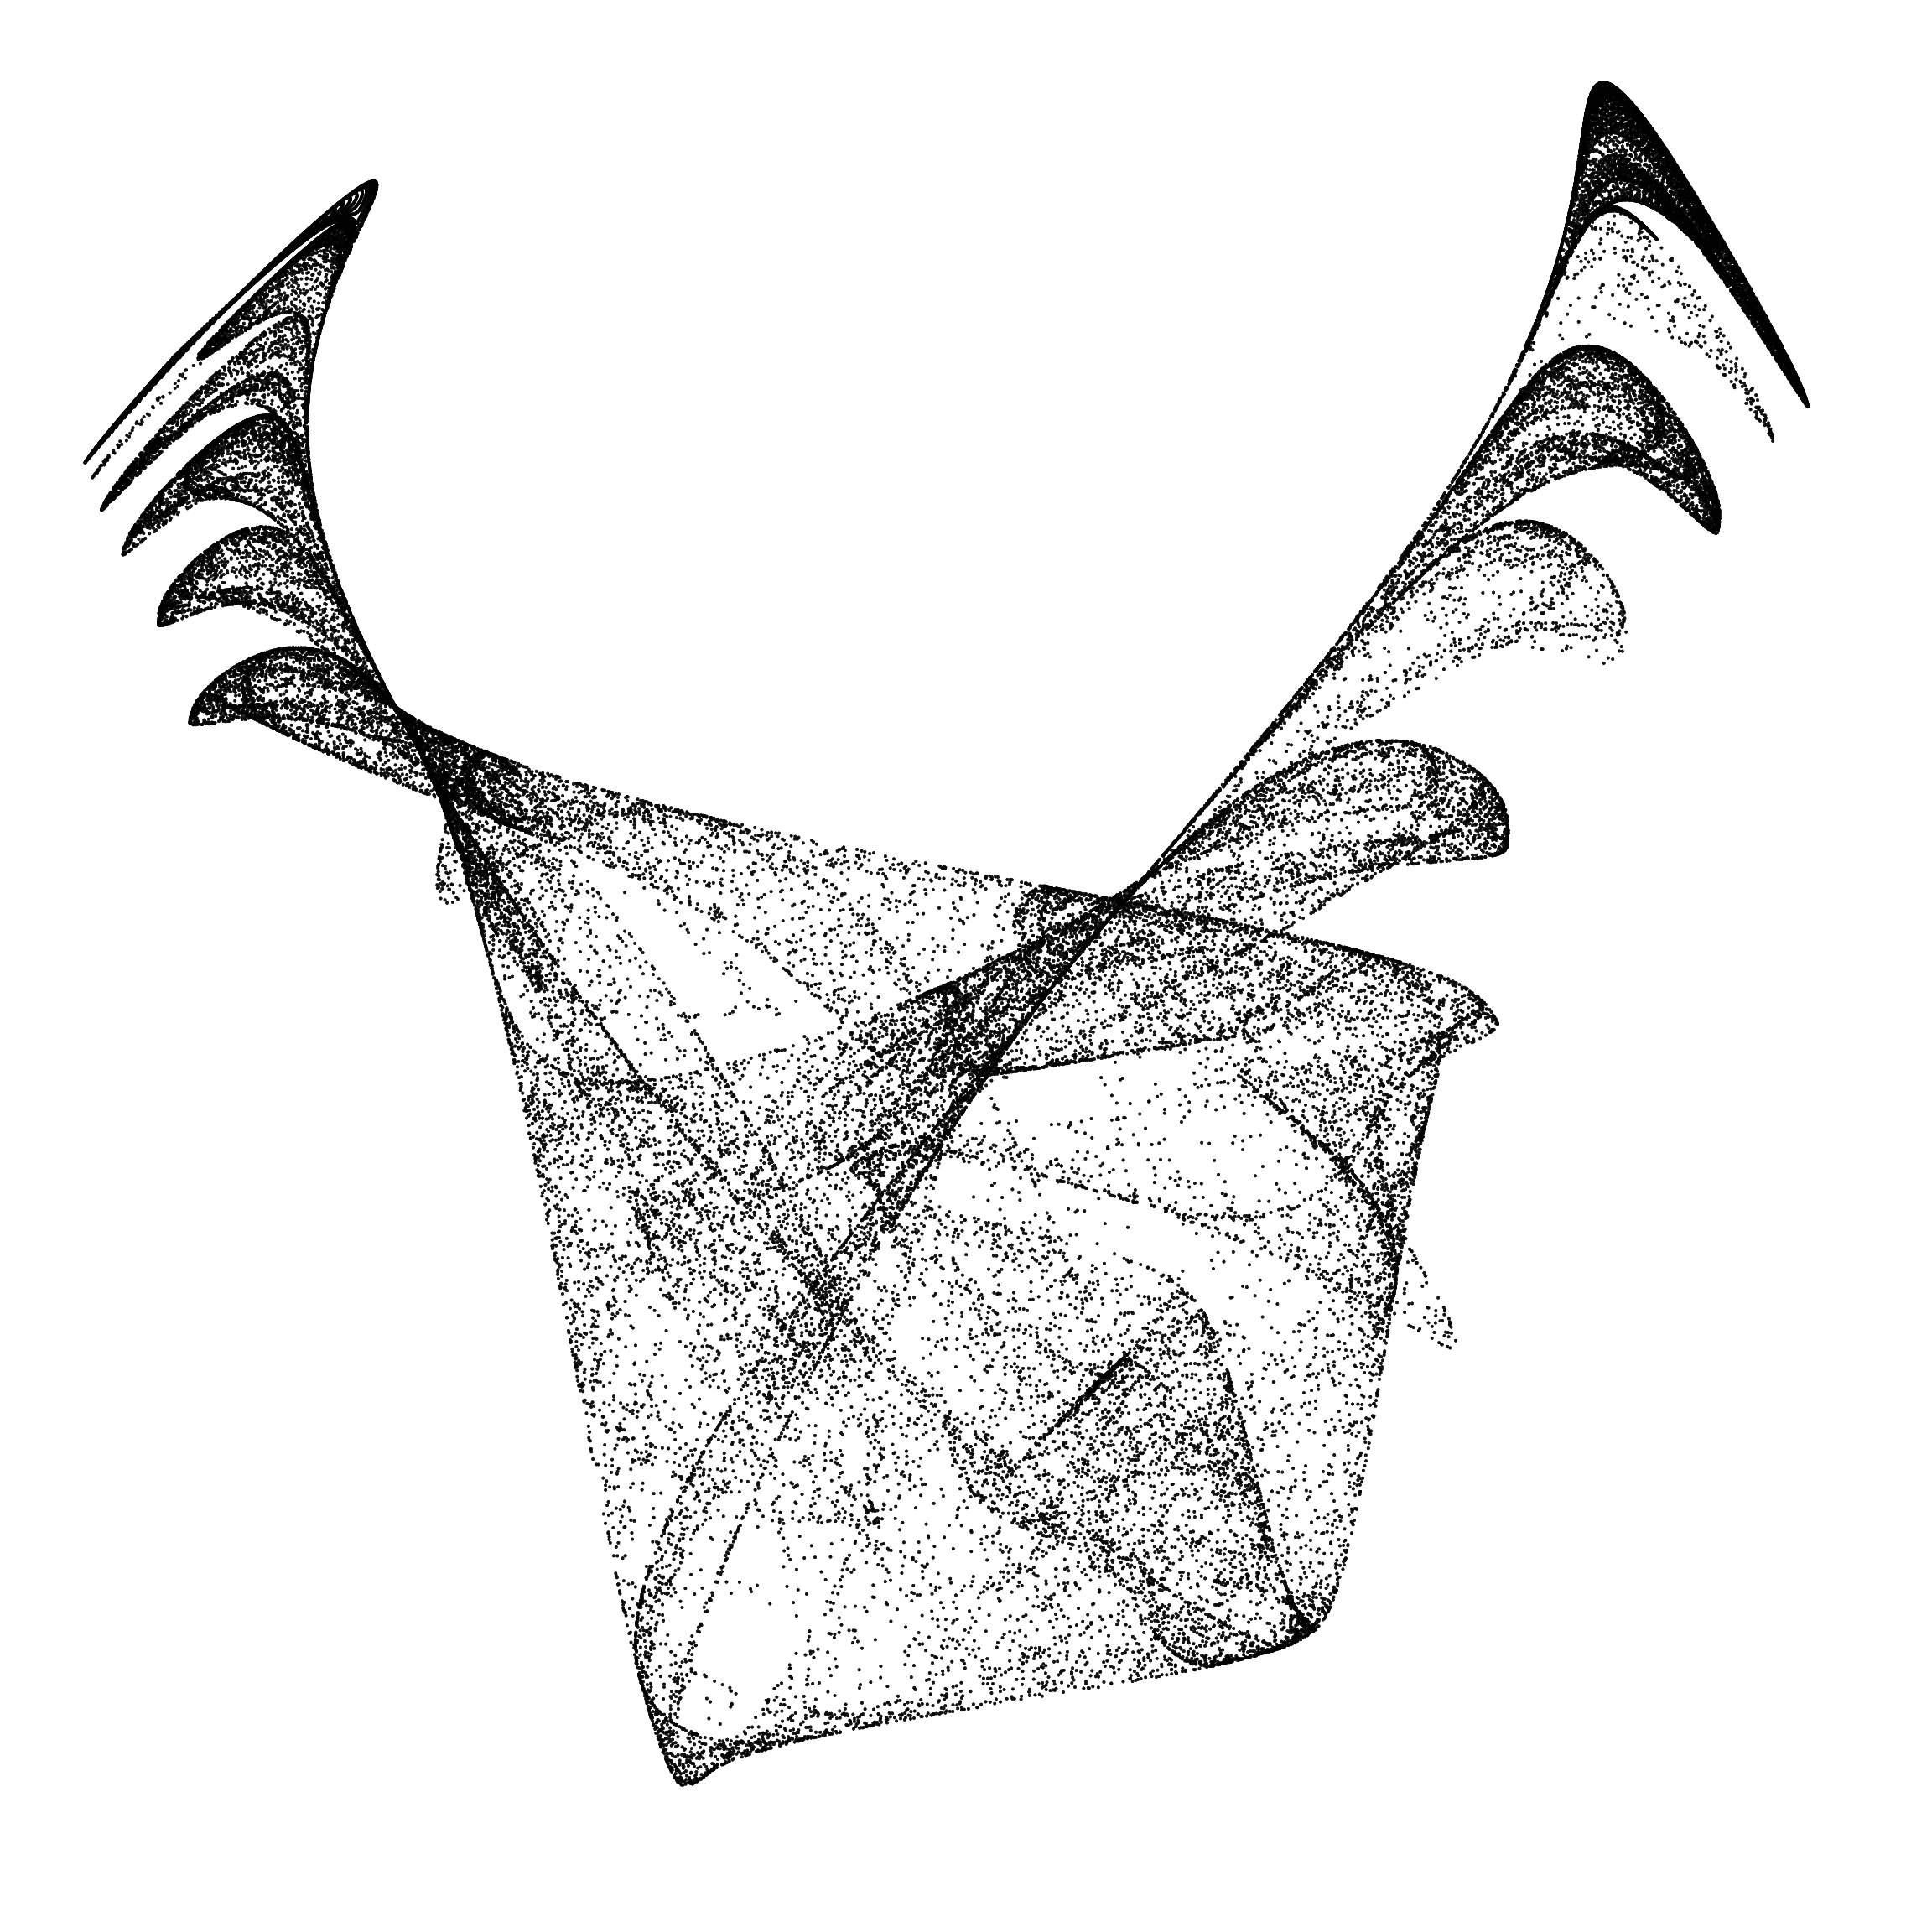
\includegraphics[height=5cm]{ifs}};
      \node[clabel,text=black,align=center] at (ifs) {Iterated \\ function \\ systems};
    \end{scope}
    \begin{scope}
      \node[cclip] (noise) at (45:0.625) {};
      \clip (noise) circle (2.5cm)
      node {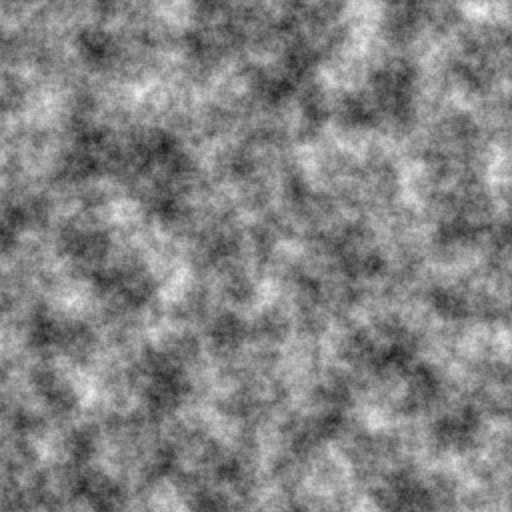
\includegraphics[height=5cm]{perlin}};
      \node[clabel,align=center,text=black] at (noise) {Noise};
    \end{scope}
    \begin{scope}
      \node[cclip] (turbulence) at (135:0.625) {};
      \clip (turbulence) circle (2.5cm)
      node {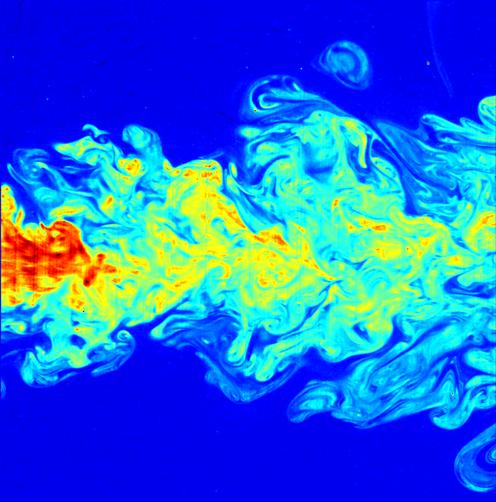
\includegraphics[height=5cm]{turbulence}};
      \node[clabel,text=black,align=center] at (turbulence) {Turbulence};
    \end{scope}
    \begin{scope}
      \node[cclip] (fern) at (-45:0.625) {};
      \clip (fern) circle (2.5cm)
      node {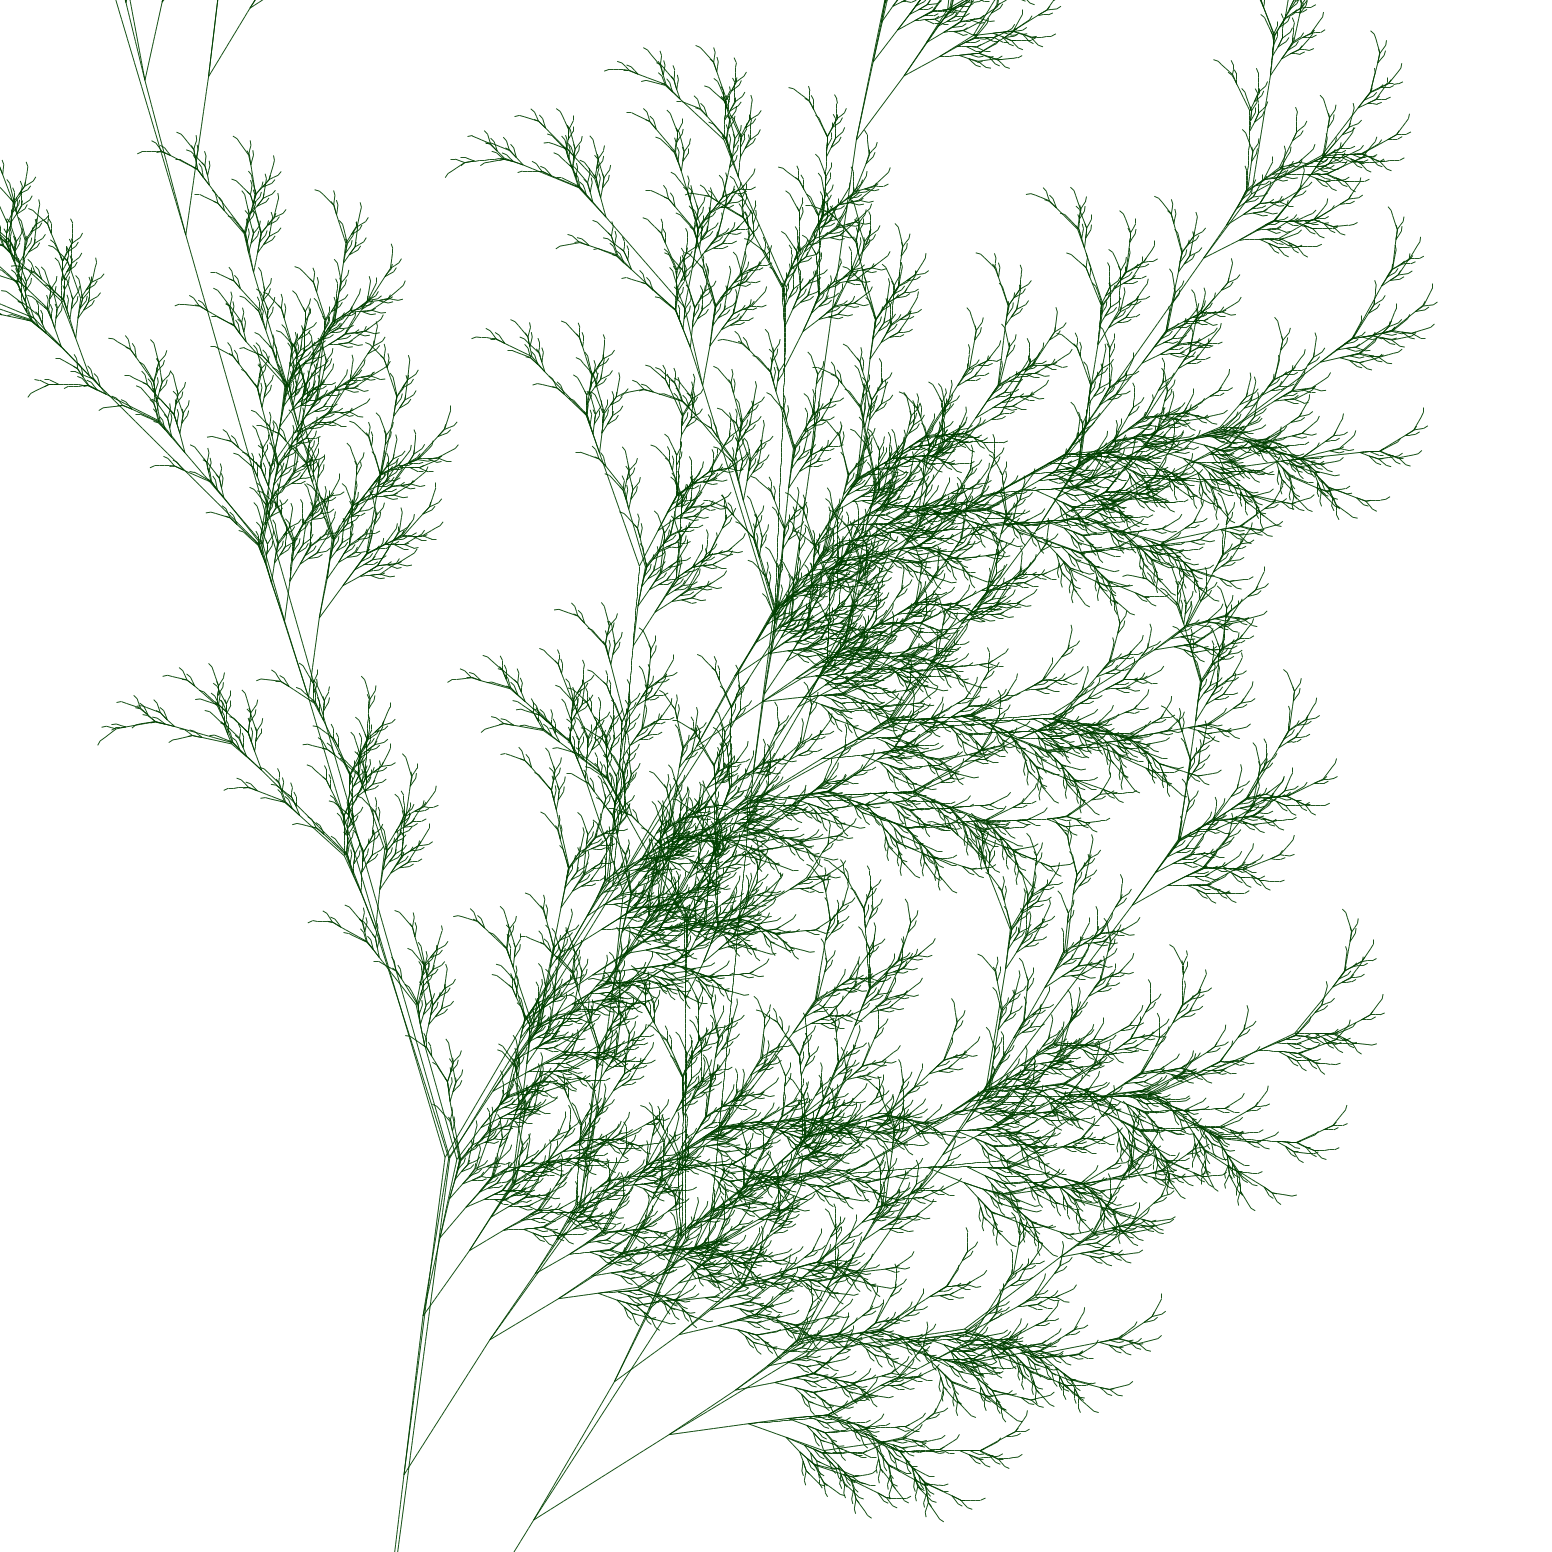
\includegraphics[height=5cm]{fern}};
      \node[clabel,text=black,align=center] at (fern) {L-systems};
    \end{scope}
    \addtocounter{beamerpauses}{3}
  \end{tikzpicture}
  };

  \node[xshift=0.666667\textwidth,yshift=0.25\textheight] at (visual world) {%
  \begin{tikzpicture}[
    visible on=<+->,
    x=7cm,
    y=7cm,
    cclip/.style = {transparent, circle, minimum size=5cm, outer sep=6pt},
    clabel/.style = {text opacity=1, inner sep=0pt, text=white, font=\bfseries, align=center}
    ]
    \node[circle, fill=black!10, inner sep=0pt,
      outer sep=0pt, minimum size=13cm]
      (graphics) at (0,0) {};
    \node[below=of graphics, inner sep=0pt, outer sep=0pt, text
      width=18cm, align=center] {\vbox{%
        These methods are \textbf{widely used} to create graphics.
        \\\vspace{0.5\baselineskip}\small
        The electric sheep ``fractal flame'' screen saver is based on
          iterated function systems.
        Noise and turbulence are combined to procedurally generate
          textures for 3D models.
        L-systems are a component of \textit{SpeedTree}, which is the
          software used to create vegetation for movies like \textit{Avatar}.
      }};
    \begin{scope}
      \node[cclip] (sheep) at (120:0.5) {};
      \clip (sheep) circle (2.5cm)
      node {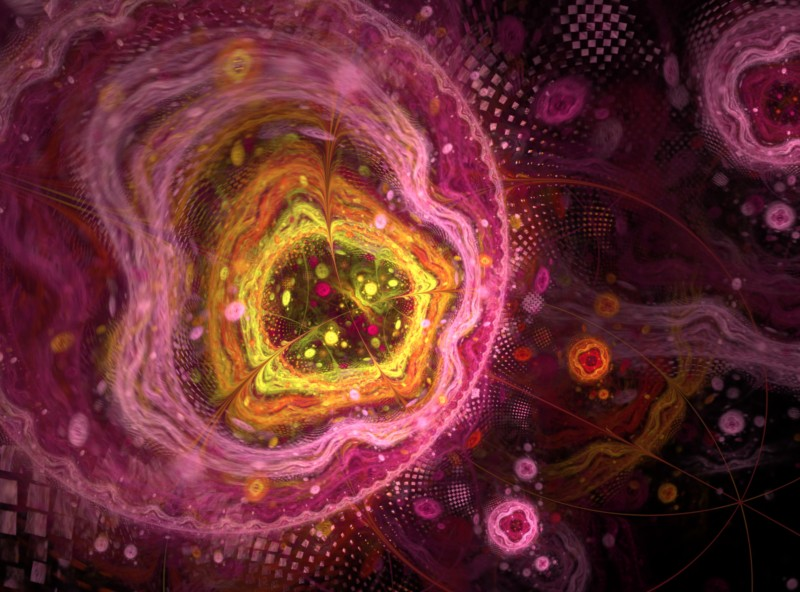
\includegraphics[height=5cm]{sheep}};
      \node[clabel] at (sheep) {Fractal \\ flame};
    \end{scope}
    \begin{scope}
      \node[cclip] (avatar) at (0:0.5) {};
      \clip (avatar) circle (2.5cm)
      node at (avatar) {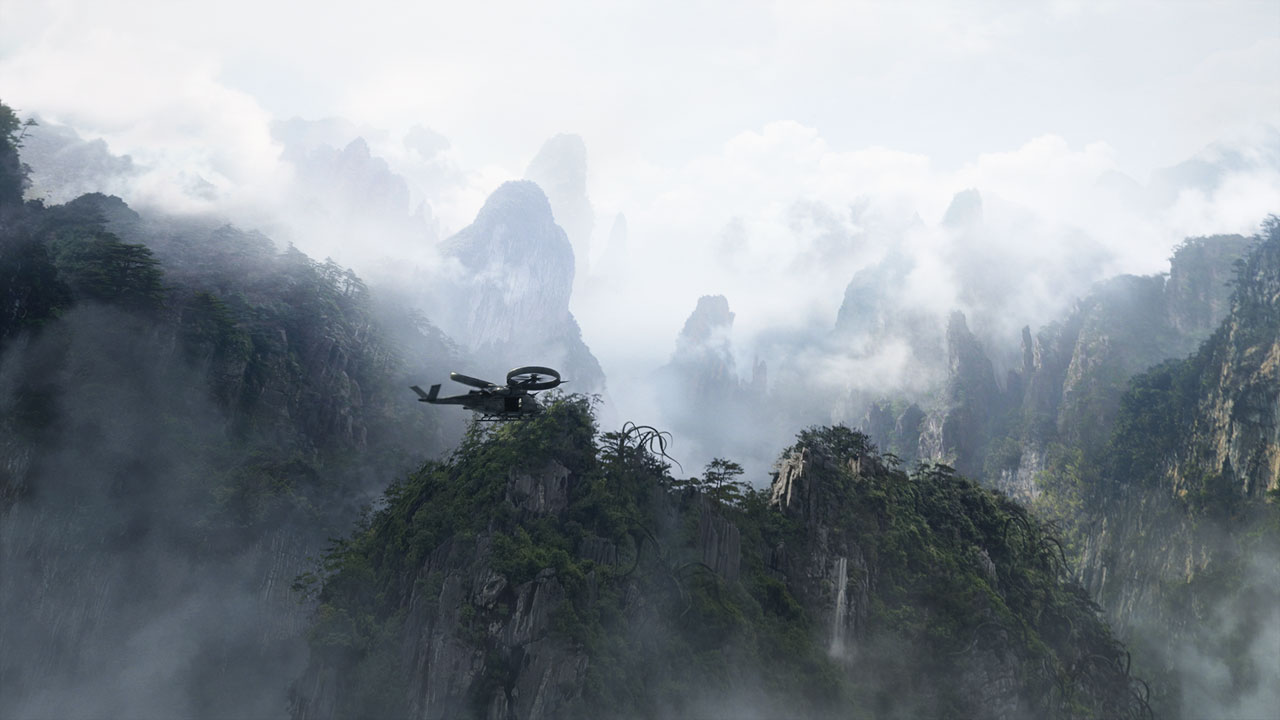
\includegraphics[height=5cm]{avatar}};
      \node[clabel,text=black] at (avatar) {Vegetation};
    \end{scope}
    \begin{scope}
      \node[cclip] (mud) at (-120:0.5) {};
      \clip (mud) circle (2.5cm)
      node {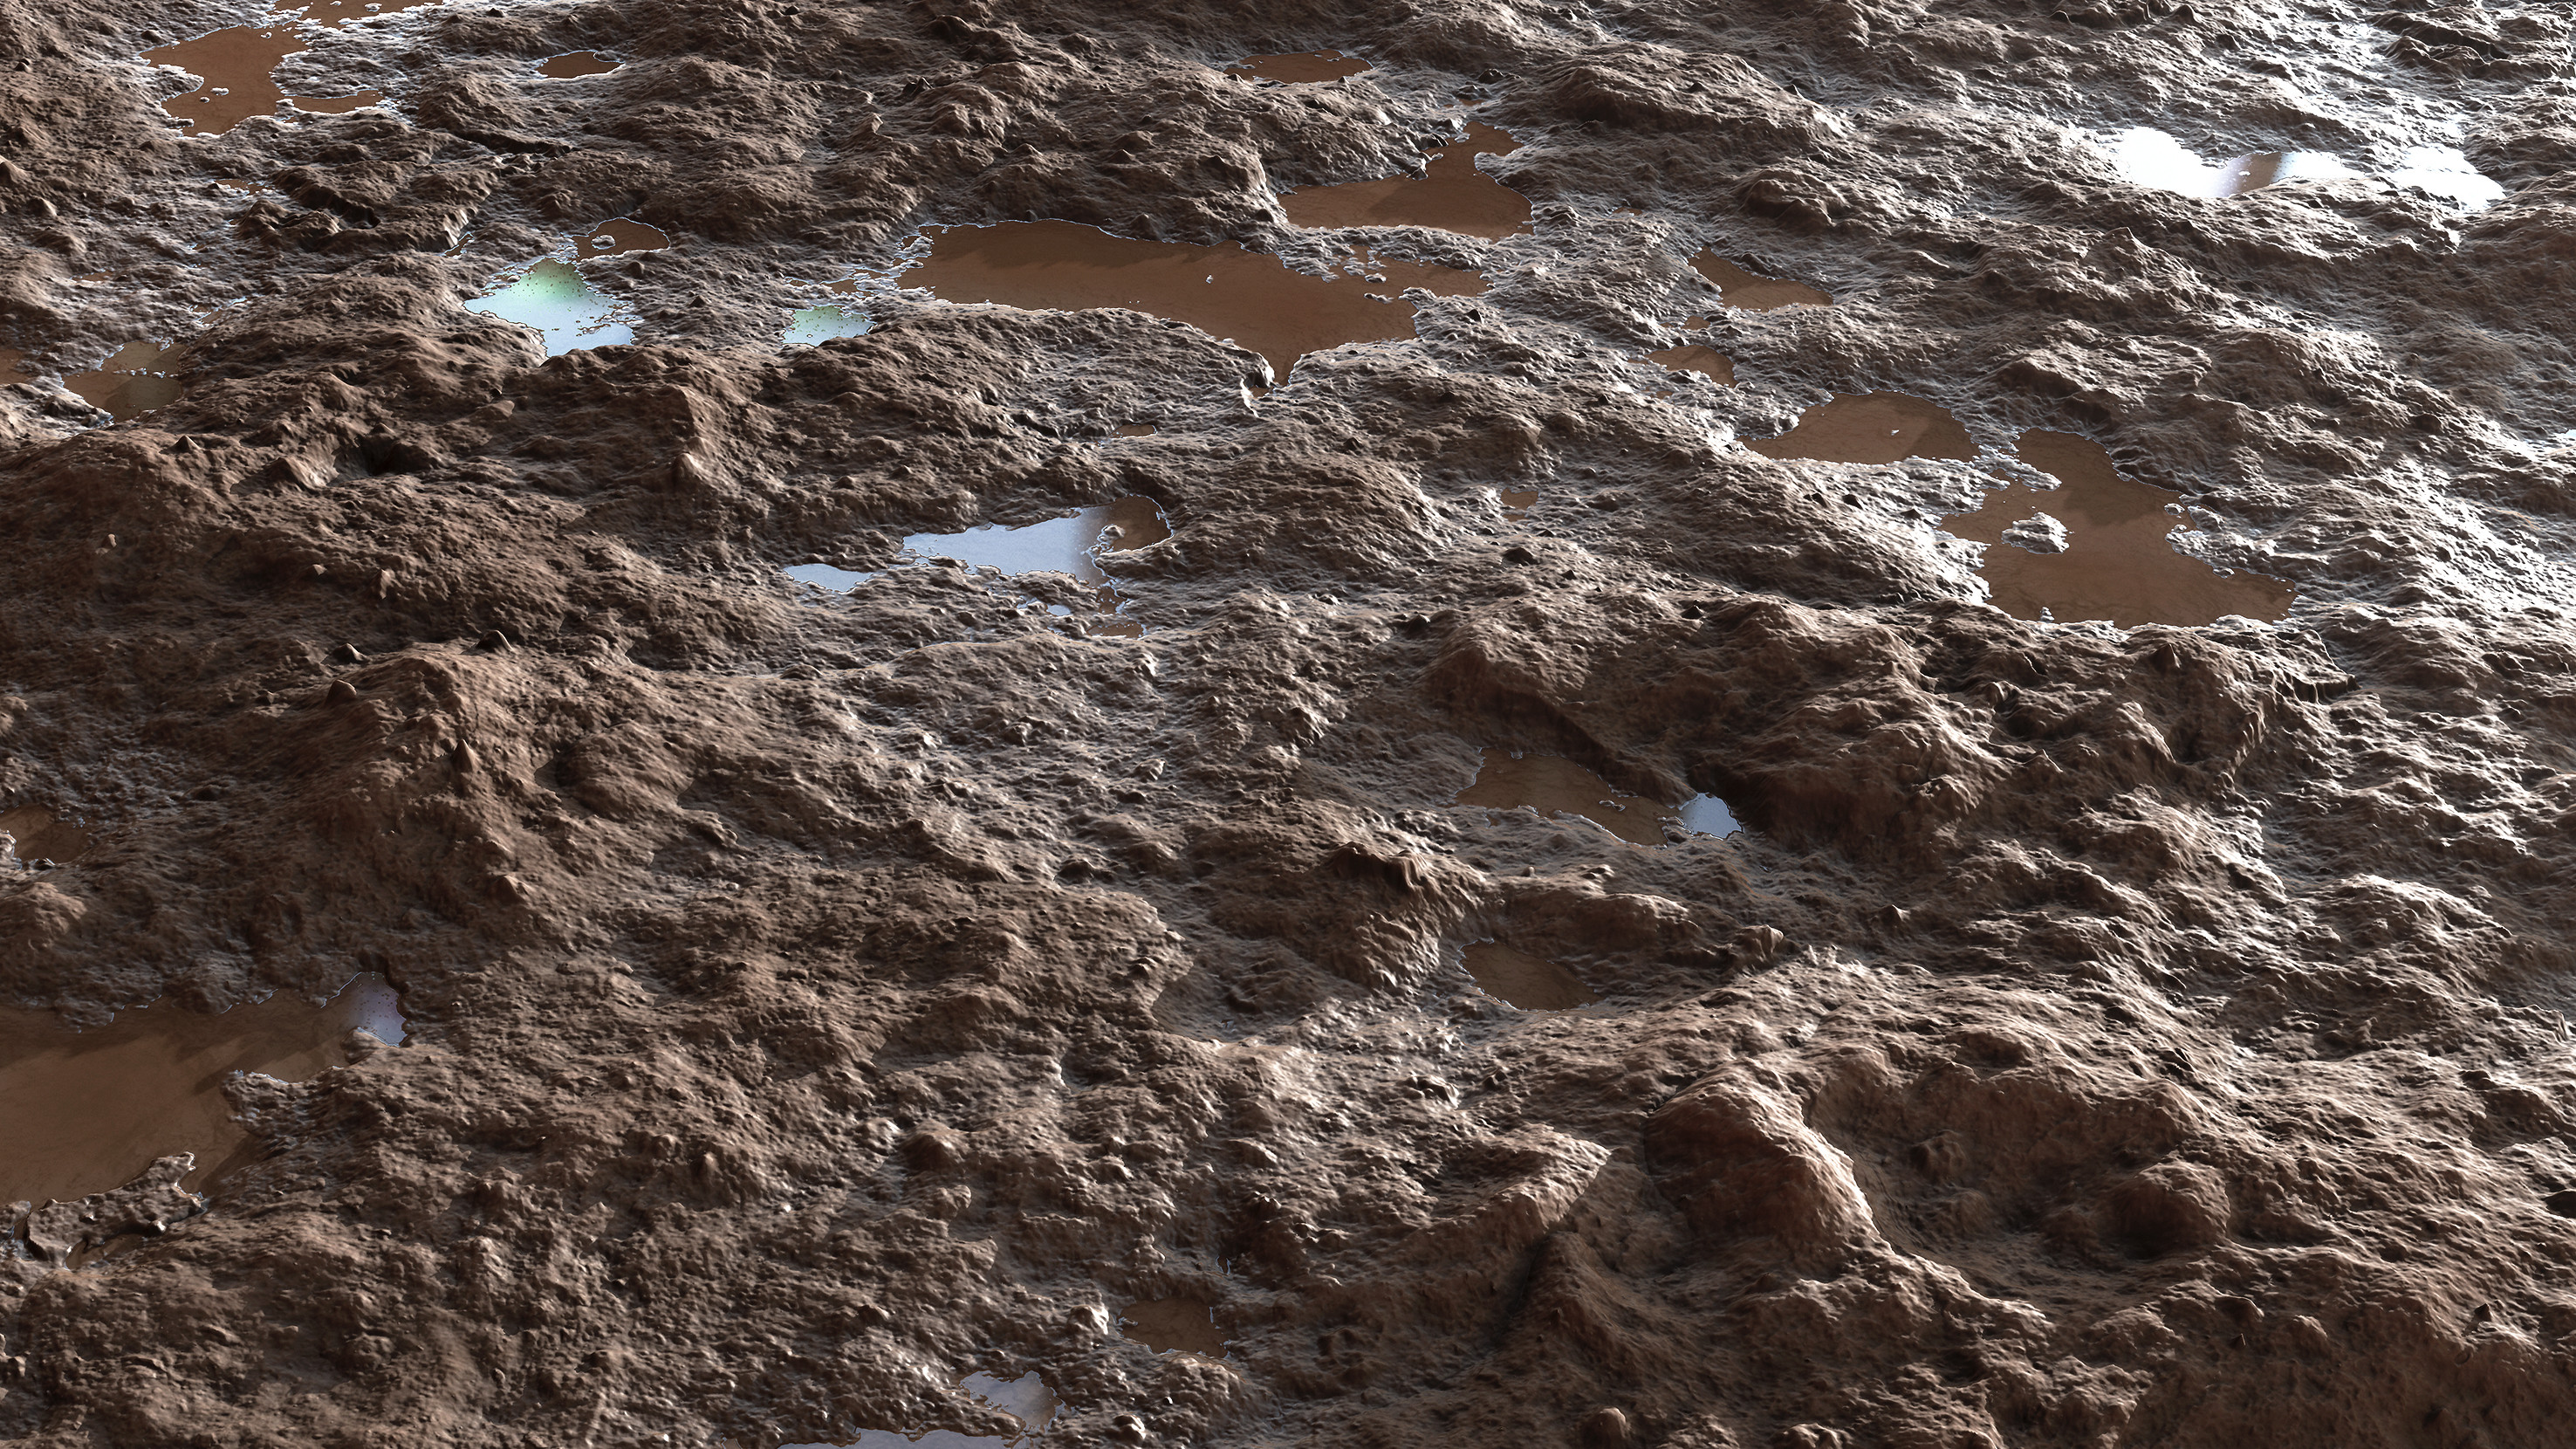
\includegraphics[height=5cm]{mud}};
      \node[clabel] at (mud) {Procedural \\ Texture};
    \end{scope}
    \addtocounter{beamerpauses}{2}
  \end{tikzpicture}
  };

  \node[xshift=0.5\textwidth,yshift=0\textheight] at (visual world) {%
  \begin{tikzpicture}[
    visible on=<+->,
    x=7cm,
    y=7cm,
    cclip/.style = {transparent, circle, minimum size=5cm, outer sep=6pt},
    clabel/.style = {text opacity=1, inner sep=0pt, text=white, font=\bfseries}
    ]
    \node[fill=black!10, inner sep=0pt,
      outer sep=0pt, minimum width=12.5cm, minimum height=6cm, rounded rectangle]
      (rfs) at (0,0) {};
    \node[below=of rfs, inner sep=0pt, outer sep=0pt, text
      width=16cm, align=center] {%
        \textbf{Receptive fields} of \textit{simple cells} in area V1 are
        modeled by space-time derivatives, and are related to smoothed
        derivatives of the light field entering the eye.
      };
    \begin{scope}
      \node[cclip] (rfmap) at (-180:0.425) {};
      \clip (rfmap) circle (2.5cm)
      node {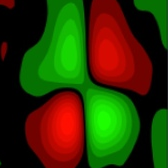
\includegraphics[height=5cm]{rf-map}};
      \node[clabel,align=center] at (rfmap) {Map};
    \end{scope}
    \begin{scope}
      \node[cclip] (rfderiv) at (0:0.425) {};
      \clip (rfderiv) circle (2.5cm)
      node {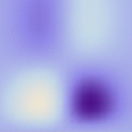
\includegraphics[height=5cm]{rf-deriv}};
      \node[clabel,align=center] at (rfderiv) {Model};
    \end{scope}
    \addtocounter{beamerpauses}{3}
  \end{tikzpicture}
  };

  \node[xshift=0.5\textwidth,yshift=-0.25\textheight] (wlresults) at (visual world) {%
  \begin{tikzpicture}[%
    visible on=<+->,
    ]
    \node (wlerr) at (0,0) {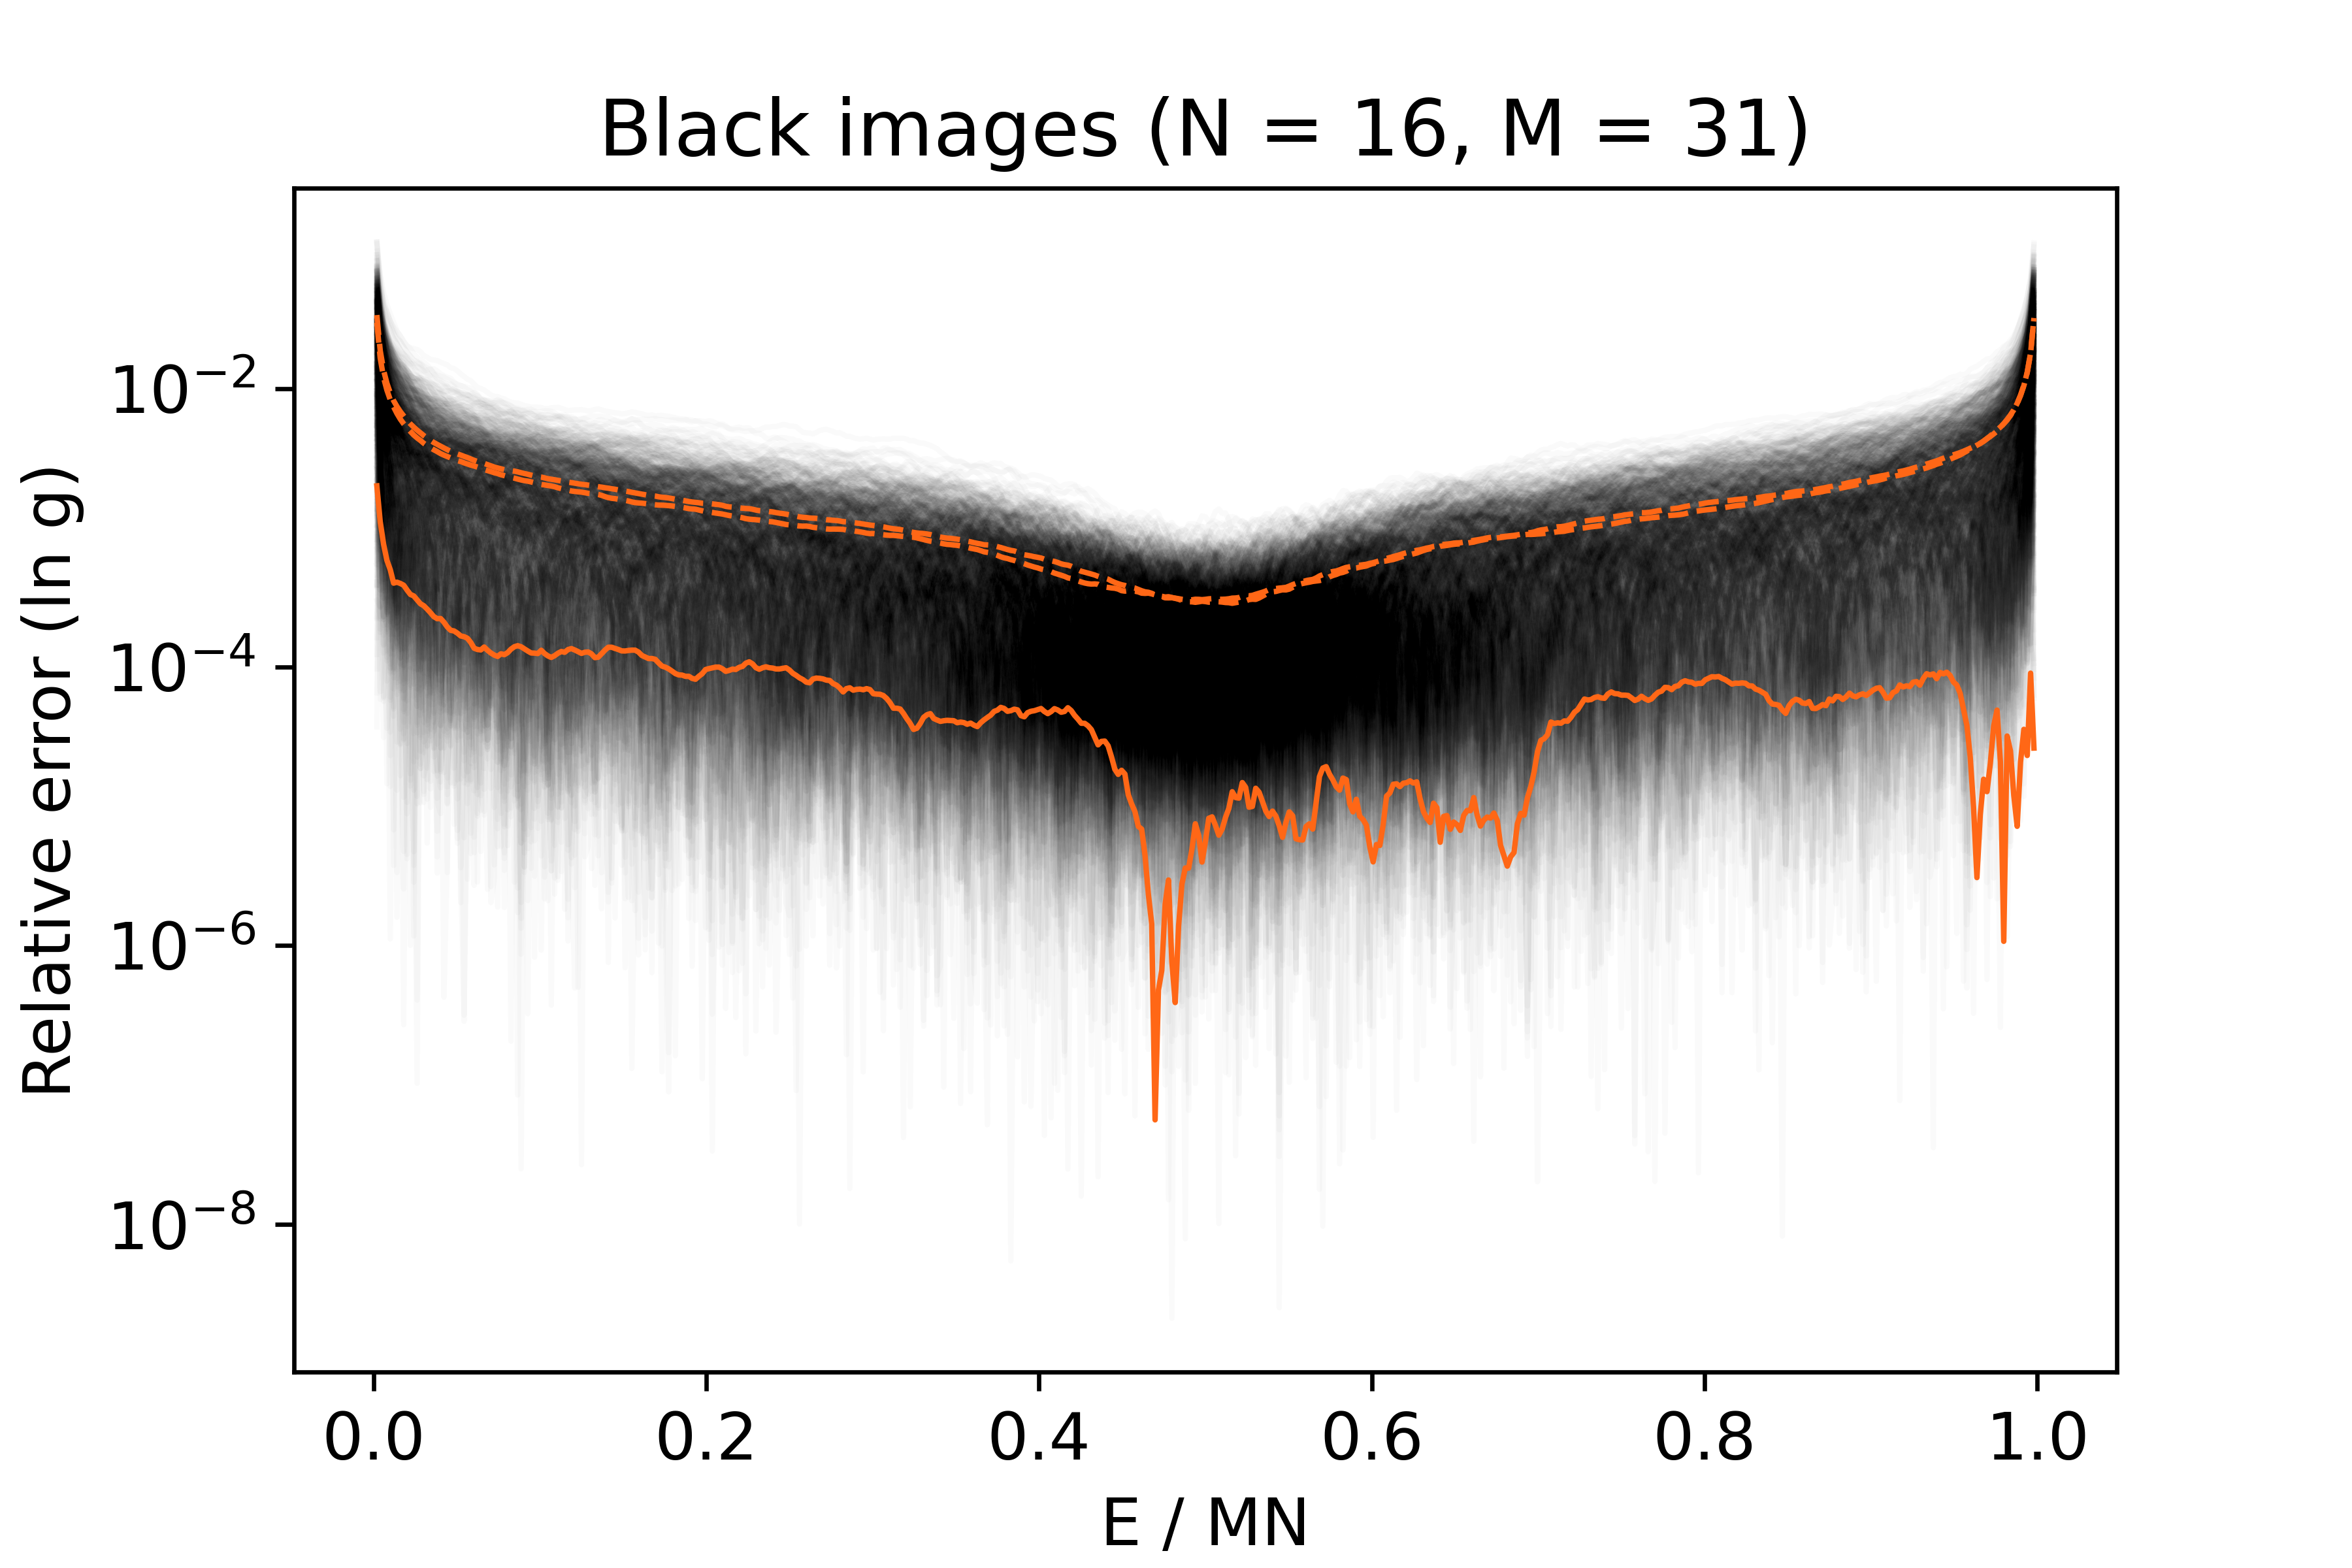
\includegraphics[width=20cm]{wanglandau-bw-relerror}};
    \node[right=-2cm of wlerr] (wles) {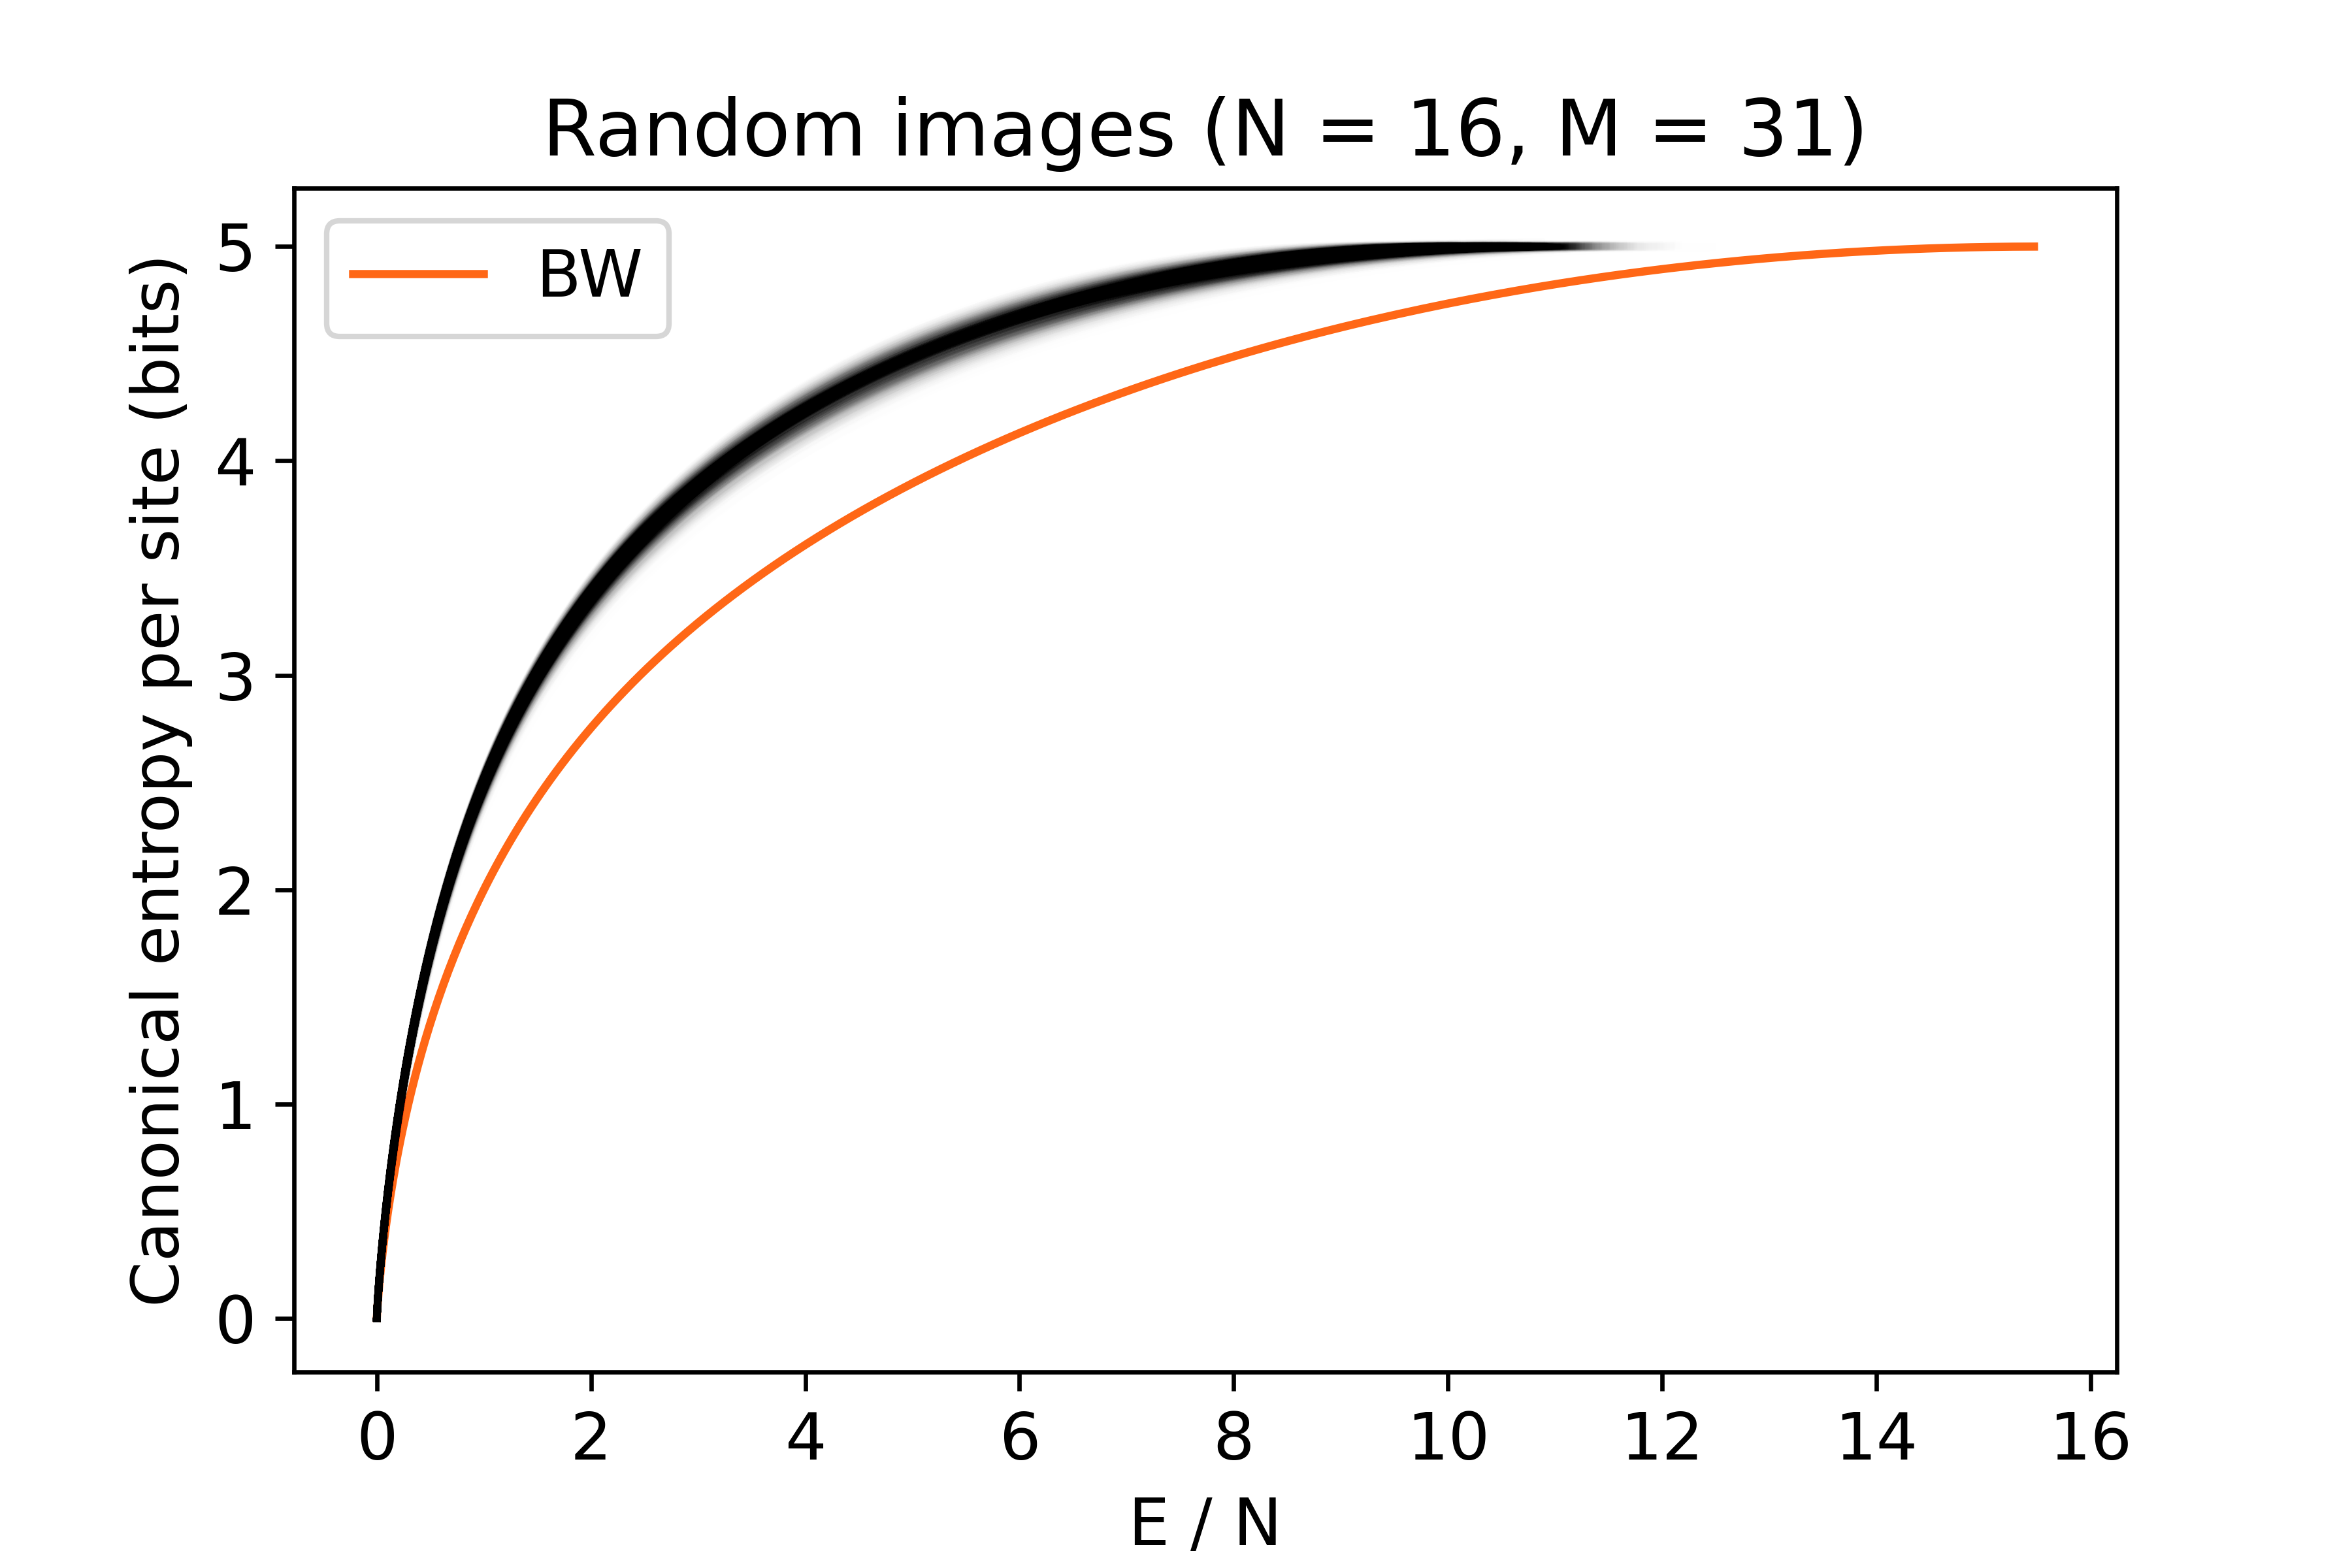
\includegraphics[width=20cm]{wanglandau-gray-ES}};
  \end{tikzpicture}
  };
  
  \node[visible on=<.->,below=-0.5ex of wlresults,align=center,text width=40cm] {%
    For a notion of lost information in an image, we may perform simulations of
    \textbf{images as discrete-level systems}, where the
    \textcolor{blue}{energy} is the sum of the differences in pixel values. The
    \textit{Wang-Landau} algorithm was implemented for images, and confirmed to
    have the expected convergence properties on \textcolor{orange}{black or
    white (BW)} images (\emph{left}). Simulations for \num{1024} random
    grayscale images (\textit{right}) reveal how entropy scales with how
    different the pixel values are (average energy).
  };

  \node[visible on=<.->,xshift=11.5cm,yshift=-1.5cm] at (wlresults) {%
  \tikzstyle{emph} = [fill=blue]
  \begin{tikzpicture}[line width=2pt, every node/.style={transform shape}]
    \node[left] at (1.25*1, 1 + 0.5) {\small$1$};
    \node[left] at (1.25*1, 5 + 0.5) {\small$M$};
    \node[below] at (1.25*1 + 0.5,1) {\small$1$};
    \node[below] at (1.25*4 + 0.5,1) {\small$N$};
    \fill[gray] (1.25*1,4) rectangle ++(1,1);
    \fill[emph] (1.25*1,3) rectangle ++(1,1);
    \fill[gray] (1.25*2,1) rectangle ++(1,1);
    \fill[emph] (1.25*2,5) rectangle ++(1,1);
    \fill[gray] (1.25*4,2) rectangle ++(1,1);
    \fill[emph] (1.25*4,4) rectangle ++(1,1);
    \draw[emph] (1.25*4 + 1, 2 + 0.5) -- ++(0.75,0);
    \draw[emph] (1.25*4 + 1, 4 + 0.5) -- ++(0.75,0);
    \draw[emph,<->] (1.25*4 + 1.5, 2 + 0.5) -- ++(0,2)
      node[midway,right]{$\Delta E_N = 2$};
    \node (ellipses) at (1.25*3 + 0.5, 3 + 0.5) {$\cdots$};
    \foreach \x in {1,2,4} {%
      \foreach \y in {1,...,5} {%
        \draw (1.25*\x,\y) rectangle ++(1,1);
      }
    }
  \end{tikzpicture}
  };

  \node[xshift=0\textwidth,yshift=-0.333333\textheight] at (visual world) {%
  \begin{tikzpicture}[%
    visible on=<+->,
    ]
    \node (entropy) {%
      $S
      = -\sum_{x \in \mathcal{X}} p(x) \ln p(x)
      = {\langle I \rangle}_X$
    };
    \node[below=-0.5ex of entropy] (kldiv) {%
      $D_{KL}(p \mathbin{\|} q)
      = \sum_{x \in \mathcal{X}} p(x) \ln \frac{p(x)}{q(x)}$
    };
    \node[below=-0.5ex of kldiv] (pfunc) {%
      $Z = \sum_{x \in \mathcal{X}} e^{-\beta E(x)}$
    };
    \node[fit=(entropy)(kldiv)(pfunc)] (ibox) {};
    \node[above=-0.5ex of ibox] {\textbf{Statistical Physics and Information Theory}};
  \end{tikzpicture}
  };
  \end{tikzpicture}
\end{frame}
\end{document}

